% 《物理实验报告模板.tex》的共同版式；所有实验模板均载入本文件。
\documentclass[UTF8,a4paper,10pt,fontset=fandol]{ctexart}
\usepackage[left=3.175cm,right=3.175cm,top=2.54cm,bottom=2.54cm]{geometry}
\usepackage{graphicx,tikz,pgfplots,needspace,adjustbox,booktabs,fancyhdr,lastpage,amsmath,amssymb,array,tabularx,longtable}
\pgfplotsset{compat=1.18}
\setlength{\parindent}{0pt}
\setlength{\parskip}{2pt}
\setlength{\headheight}{18pt}
\linespread{1}
\newcommand{\SetField}[2]{\expandafter\def\csname reportfield@#1\endcsname{#2}}
\makeatletter
\newcommand{\Field}[2][1.35cm]{%
  \ifcsname reportfield@#2\endcsname
    \expandafter\ifx\csname reportfield@#2\endcsname\@empty
      \underline{\makebox[#1]{\strut}}%
    \else\csname reportfield@#2\endcsname\fi
  \else\underline{\makebox[#1]{\strut}}\fi}
\makeatother
\newcommand{\MathField}[2][1.35cm]{%
  \ifcsname reportfield@math_#2\endcsname
    \csname reportfield@math_#2\endcsname
  \else\text{\Field[#1]{#2}}\fi}
\newcommand{\coverfield}[2]{%
  \noindent{\heiti\fontsize{18pt}{48pt}\selectfont
  \makebox[3.3cm][l]{#1}\underline{\makebox[8.8cm][c]{\Field[0pt]{#2}}}\par}}
\newcommand{\bindingline}[1][2.85]{%
  \begin{tikzpicture}[remember picture,overlay]
    \foreach \i in {0,...,38}{%
      \pgfmathsetmacro{\bindingy}{-#1-0.52*\i}%
      \ifnum\i=13\relax
        \node[inner sep=0pt] at ([xshift=1.05cm,yshift=\bindingy cm]current page.north west) {\songti\fontsize{10.5pt}{10.5pt}\selectfont 装};
      \else\ifnum\i=19\relax
        \node[inner sep=0pt] at ([xshift=1.05cm,yshift=\bindingy cm]current page.north west) {\songti\fontsize{10.5pt}{10.5pt}\selectfont 订};
      \else\ifnum\i=25\relax
        \node[inner sep=0pt] at ([xshift=1.05cm,yshift=\bindingy cm]current page.north west) {\songti\fontsize{10.5pt}{10.5pt}\selectfont 线};
      \else
        \pgfmathsetmacro{\bindingtop}{\bindingy+0.20}%
        \pgfmathsetmacro{\bindingbottom}{\bindingy-0.20}%
        \draw[line width=0.35pt,dash pattern=on 1.2pt off 1.8pt]
          ([xshift=1.05cm,yshift=\bindingtop cm]current page.north west)
          -- ([xshift=1.05cm,yshift=\bindingbottom cm]current page.north west);
      \fi\fi\fi}
  \end{tikzpicture}%
}
% 装订线印在每一页正文和原始数据页，续页也沿用母模板样式。
\newif\ifreportbinding
\AddToHook{shipout/foreground}{\ifreportbinding\bindingline\fi}
\fancypagestyle{report}{\fancyhf{}\fancyfoot[C]{第\thepage 页\quad 共\pageref{LastPage}页}\renewcommand{\headrulewidth}{0.4pt}}
\fancypagestyle{record}{\fancyhf{}\fancyhead[C]{原始数据记录单}\fancyfoot[C]{第\thepage 页\quad 共\pageref{LastPage}页}\renewcommand{\headrulewidth}{0.4pt}}
\newcommand{\ReportCover}[1]{%
  \thispagestyle{empty}\vspace*{1.0cm}
  \begin{center}
    
\includegraphics[width=8.184cm]{tongji_logo.jpeg}\par
    {\bfseries\fontsize{18pt}{24pt}\selectfont TONGJI UNIVERSITY\par}
    \vspace{1.5cm}{\heiti\fontsize{36pt}{44pt}\selectfont 物理实验报告\par}
  \end{center}
  \vspace{1.5cm}
  \coverfield{实验名称}{experiment}
  \coverfield{学生姓名}{student}
  \coverfield{学\hspace{1em}号}{student_id}
  \coverfield{组\hspace{1em}号}{group}
  \coverfield{实验日期}{date}
  \clearpage\reportbindingtrue\pagestyle{report}
  \begin{center}{\heiti\fontsize{14pt}{40pt}\selectfont #1\par}\end{center}}
\newcommand{\ReportSection}[1]{\Needspace{4\baselineskip}\par\vspace{0.35\baselineskip}{\heiti #1}\par}
\newcommand{\ReportSubsection}[1]{\Needspace{3\baselineskip}\par\vspace{0.2\baselineskip}{\bfseries #1}\par}
\newif\ifreportimages
\newcommand{\ReportRecord}{%
  \clearpage\thispagestyle{record}
  \vspace*{0.6cm}%
  \ifreportimages\else（请将教师签字的实验数据记录单完整拍照粘贴至此处。）\fi
}

% ===== 数据输入区开始 =====
\SetField{experiment}{密立根油滴实验}
% 后端以 \SetField{字段名}{值} 填入数据；缺省值保持空白。
% 母模板封面字段：\Field{experiment} \Field{student} \Field{student_id} \Field{group} \Field{date}
% ===== 数据输入区结束 =====
\begin{document}\fontsize{10.5pt}{20pt}\selectfont
\ReportCover{密立根油滴实验}
\ReportSection{实验目的}
1. 观察带电油滴在重力和电场力作用下的运动，用平衡电压与下降时间估计油滴电荷量。\par
2. 理解电荷量子化假设 $q_i\approx n_i e$，并用多颗油滴检查整数倍关系。\par
3. 分别用反向验证、图解拟合和过原点最小二乘法估计元电荷，比较三种处理方式。\par
4. 练习识别布朗运动、油滴蒸发和计时误差对结果的影响。\par
\ReportSection{实验原理}
\ReportSubsection{3.1 静态平衡法}
用喷雾器将油滴喷入两块相距为 $d$ 的水平放置的平行板之间，如图 8.3.1 所示，油滴在喷射时由于摩擦会带有电荷。设油滴的质量为 $m$，所带电量为 $Q$，两极板间所加的电压为 $U$，则油滴在平行板间将同时受到两个力的作用，一个是重力 $mg$，一个是静电力 $QE=QU/d$，两个力的方向如图所示。
\begin{center}
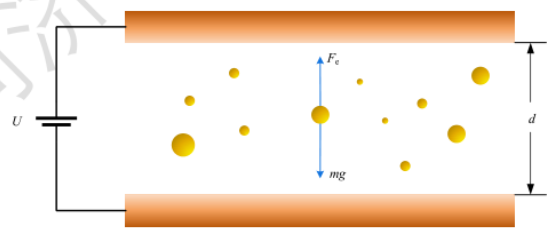
\includegraphics[width=9cm]{figures/millikan-static-source.png}\par
{\small 图 8.3.1 静态法测量原理图}
\end{center}
如果调节两极板间的电压 $U$，可使两力相互抵消而达到平衡，此时 $mg=QU/d$，故有
\begin{equation}Q=mg\frac{d}{U}.\tag{8.3.1}\end{equation}
平行板未加电压时，油滴受重力作用而加速下降，但空气对油滴所产生的黏滞阻力 $F_r$ 与速度成正比。油滴走了一段距离到达某一速度 $v_g$ 后，黏滞阻力与重力平衡（空气浮力忽略不计），油滴将匀速下降，由斯托克斯定律可知
\begin{equation}F_r=6\pi a\eta v_g=mg.\tag{8.3.2}\end{equation}
式中，$\eta$ 是空气的黏度，$a$ 是油滴的半径（由于表面张力的原因，油滴近乎呈小球状）。设油滴的密度为 $\rho$，则油滴的质量 $m$ 可表示为
\begin{equation}m=\frac{4}{3}\pi a^3\rho.\tag{8.3.3}\end{equation}
合并式 (8.3.2) 和式 (8.3.3)，得油滴的半径为
\begin{equation}a=\sqrt{\frac{9\eta v_g}{2\rho g}}.\tag{8.3.4}\end{equation}
对于半径很小的油滴（直径约为 $10^{-6}$ m），空气已经不能视为连续介质。考虑空气分子的平均自由程与大气压强成正比等因素，斯托克斯定律应修正为
\begin{equation}F_r=\frac{6\pi a\eta v_g}{1+\dfrac{b}{pa}}.\tag{8.3.5}\end{equation}
式中，$b$ 为一修正常数，$b=8.22\times10^{-3}$ m$\cdot$Pa，$p$ 为大气压强，单位为 Pa。于是得
\begin{equation}a=\sqrt{\frac{9\eta v_g}{2\rho g}\left(\frac{1}{1+\dfrac{b}{pa}}\right)}.\tag{8.3.6}\end{equation}
上式根号中还包含油滴的半径 $a$，但因它是处于修正项中，不需要十分精确，故它仍可用式 (8.3.4) 计算。将式 (8.3.5) 代入式 (8.3.3)，得
\begin{equation}m=\frac{4}{3}\pi\left[\frac{9\eta v_g}{2\rho g}\frac{1}{1+\dfrac{b}{pa}}\right]^{3/2}\rho.\tag{8.3.7}\end{equation}
当两极板间的电压 $U=0$ 时，设油滴匀速下降的距离为 $l$，时间为 $t$，则
\begin{equation}v_g=\frac{l}{t}.\tag{8.3.8}\end{equation}
由式 (8.3.1)、(8.3.6)、(8.3.7) 得
\begin{equation}Q=\frac{18\pi}{\sqrt{2\rho g}}\left[\frac{\eta l}{t\left(1+\dfrac{b}{pa}\right)}\right]^{3/2}\frac{d}{U}.\tag{8.3.9}\end{equation}
式中 $\eta$、$l$、$\rho$、$g$、$d$ 均为与实验条件、仪器有关的参量，均为已知量，只需测出平衡电压 $U_n$ 和油滴匀速下落 $l$ 所用时间 $t$，即可求出油滴带电量 $Q$。
将式 (8.3.4) 代入式 (8.3.9)，并引入 $k$ 和 $k'$ 后计算式为
\begin{equation}Q=\frac{k}{\left[t\left(1+k'\sqrt{t}\right)\right]^{3/2}}\frac{1}{U}.\tag{8.3.10}\end{equation}
式中
\begin{equation}k=\frac{18\pi}{\sqrt{2\rho g}}(\eta l)^{3/2}d,\tag{8.3.11}\end{equation}
和
\begin{equation}k'=\frac{b}{p}\sqrt{\frac{2\rho g}{9\eta l}}.\tag{8.3.12}\end{equation}
实验发现，对于同一油滴，如果我们改变它所带的电量，则能够使油滴达到平衡的电压 $U$，必须是某些特定的值 $U_n$，这表示与它相对应的电量 $Q$ 是不连续的，即
\begin{equation}Q_n=ne=mg\frac{d}{U_n}.\tag{8.3.13}\end{equation}
式中，$n=\pm1,\ \pm2,\ \ldots$。对于不同的油滴，可以发现有同样的规律，而且 $e$ 值是 $Q_1,Q_2,\ldots,Q_n$ 的最大公约数，这就证明了电荷的不连续性，并存在着最小的带电单位，即电子的电荷值 $e$。
\ReportSubsection{实验参数与计算常数}
实验参数如表 8.3.1 所示。
\begin{center}\small
表 8.3.1 密立根油滴实验参数表\par
\renewcommand{\arraystretch}{1.45}
\begin{tabular}{p{8cm}|p{4cm}}\toprule
\multicolumn{1}{c|}{名称} & \multicolumn{1}{c}{参数}\\\midrule
极板间距 $d$(m) & $5\times10^{-3}$\\
油滴匀速下落距离 $l$(m) & $1.6\times10^{-3}$\\
空气黏度 $\eta$(kg$\cdot$m$^{-1}\cdot$s$^{-1}$) & $1.83\times10^{-5}$\\
20$^\circ$C 钟表油密度 $\rho_1$(kg$\cdot$m$^{-3}$) & $981$\\
标准状况下空气密度 $\rho_2$(kg$\cdot$m$^{-3}$) & $1.2928$\\
上海地区重力加速度 $g$(m$\cdot$s$^{-2}$) & $9.794$\\
修正常数 $b$(m$\cdot$Pa) & $8.23\times10^{-3}$\\
标准大气压强 $p$(Pa) & $1.01325\times10^5$\\\bottomrule
\end{tabular}\end{center}
将以上参数代入公式 (8.3.11) 和 (8.3.12) 得
\begin{equation}k=0.928\times10^{-14}\ \mathrm{kg\cdot m^2\cdot s^{-1/2}},\tag{8.3.17}\end{equation}
和
\begin{equation}k'=0.0226\ \mathrm{s^{-1/2}}.\tag{8.3.18}\end{equation}
将 $k$ 和 $k'$ 代入式 (8.3.10) 得
\begin{equation}Q=\frac{0.928\times10^{-14}}{\left[t\left(1+0.0226\sqrt{t}\right)\right]^{3/2}}\frac{1}{U_n}.\tag{8.3.19}\end{equation}
显然，由于油滴的密度 $\rho$、空气的黏度 $\eta$ 都是温度的函数，大气压强 $p$ 又随实验地点和条件的变化而变化。因此，上式的计算是近似的。一般情况下，由于它们引起的误差仅 1\% 左右，可以使计算大为简化，当然也可以实验时实际参数代入公式进行计算。
\ReportSubsection{4.2 元电荷的测量方法}
密立根油滴法测量电子电量，必须通过实验取得大量的实验数据，综合地运用分析统计的方法，才能正确地估算出实验结果。常见方法有模糊统计法、反向验证法和最小二乘法等。
\ReportSubsection{（1）模糊统计法}
假如通过测量并计算得到一组（20 个以上）油滴所带的电量值 $Q_1,Q_2,Q_3,\ldots,Q_m$。把这些数据标在数轴上，通过图形可以直观地看到数据形成疏密有致、一簇一簇的有序分布，如图 8.3.5 所示。其中间距较大的应该是基本电荷数 $n$ 的差异，而间距较小的应该是测量随机误差形成的差异。对同一簇数据求平均，可得一组按不同基本电荷数排列的数据 $q_1,q_2,\ldots,q_n$。
\begin{center}
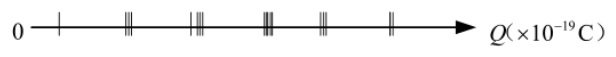
\includegraphics[width=10cm]{figures/millikan-charge-axis-source.png}\par
{\small 图 8.3.5 油滴电荷量数轴示意图}
\end{center}
对这些数据进行逐差处理，也即 $e_1=Q_2-Q_1$，$e_2=Q_3-Q_2$，$\ldots$，$e_n=Q_n-Q_{n-1}$。只要测量数据足够多，通过分析差值结果，可以得出结论，最小差值 $e$ 的平均值是电子电量的最佳估计值。以上得到的结果仅是一个粗略的估计值。
\ReportSubsection{（2）反向验证法}
将油滴所带的电量值 $Q_i\ (i=1,2,\ldots,m)$ 分别除以公认的电子电荷 $e_0=1.602\times10^{-19}$ C，把得到的商按修约规则取整数可得第 $i$ 颗油滴所带的基本电荷数 $n_i$。
\begin{equation}n_i=\frac{Q_i}{e_0}\quad\text{（取整）}.\tag{8.3.20}\end{equation}
再用 $n_i$ 去除 $Q_i$ 得到的值即为实验测量的电子电荷值 $e_i$。偏差为
\begin{equation}\Delta e_i=e_i-e_0.\tag{8.3.21}\end{equation}
$m$ 个油滴电子电荷平均值
\begin{equation}\bar e_i=\frac{1}{m}\sum_{i=1}^{m}\frac{Q_i}{n_i}.\tag{8.3.22}\end{equation}
不确定度
\begin{equation}U_e=t\sqrt{\frac{\sum_{i=1}^{m}(\Delta e_i)^2}{m(m-1)}}.\tag{8.3.23}\end{equation}
也可以通过绘制 $Q$--$n$ 关系图，求出直线的斜率 $\Delta Q/\Delta n$，即电荷值。
\ReportSubsection{（3）最小二乘法}
设 $y_i=Q_i\ (i=1,2,\ldots,m)$，拟合值 $\hat y_i=en_i$，则
\begin{equation}y_i-\hat y_i=Q_i-en_i.\tag{8.3.24}\end{equation}
式 (8.3.24) 等式两边求平方和，可得
\begin{equation}S=\sum_{i=1}^{m}(y_i-\hat y_i)^2=\sum_{i=1}^{m}(Q_i-en_i)^2.\tag{8.3.25}\end{equation}
要使 $S$ 为最小值，可以 $e$ 作为变量，对方程左式求导，并令导数为 0，以期求得使 $\sum_i(Q_i-en_i)^2$ 为最小值的 $e$，也即电子电量实验值 $e$ 的最优值，即
\begin{equation}\frac{\mathrm dS}{\mathrm de}=\frac{\mathrm d}{\mathrm de}\sum_{i=1}^{m}(Q_i-en_i)^2=0.\tag{8.3.26}\end{equation}
求导数，得
\begin{equation}\sum_{i=1}^{m}n_iQ_i-\sum_{i=1}^{m}en_i^2=0.\tag{8.3.27}\end{equation}
解方程得到电子电量最优值为
\begin{equation}e=\frac{\sum_{i=1}^{m}n_iQ_i}{\sum_{i=1}^{m}n_i^2}.\tag{8.3.28}\end{equation}
其不确定度为
\begin{equation}U_e=t\sqrt{\frac{\sum_{i=1}^{m}(Q_i/n_i-e)^2}{m(m-1)}}.\tag{8.3.29}\end{equation}
\Needspace{8\baselineskip}
\ReportSection{实验内容}
\ReportSubsection{观测准备}
1. 检查油滴盒清洁、照明、显微镜调焦和极板电压零点；喷入少量油雾，选取孤立且运动缓慢的油滴。\par
2. 标定目镜中的固定下降距离。关闭电场，待油滴运动稳定后计时；同一滴重复四次，若轨迹偏离或油滴消失，应重新选滴。\par
\ReportSubsection{平衡与重复测量}
3. 逐渐增大电压，使油滴尽可能悬浮，记录平衡电压。对多颗油滴重复下降计时与电压测量。\par
4. 分别计算 $q_i$、整数 $n_i$ 和 $\frac{q_i}{n_i}$；绘制散点与拟合直线，比较反向验证值、图解斜率和最小二乘结果。
\ReportSection{实验仪器}
密立根油滴仪（油滴盒、电极板、照明及显微镜）、喷油器、计时器和直流高压电源。极板间距、空气黏度与修正常数已包含在仪器给定的计算常数中。
\ReportSection{7 数据记录与处理}
\ReportSubsection{7.1 静态平衡法}
\ReportSubsection{（1）模糊统计法}
选择合适的油滴，每颗油滴重复测量 4 组下降时间 $t$ 和平衡电压 $U$，下降八格，即 $l=1.6$ mm。计算油滴所带电荷量 $Q_i$，填入表 8.3.2。每滴采用四次下降时间和平衡电压的均值。
\begin{center}\small\renewcommand{\arraystretch}{1.28}
表 8.3.2 静态平衡法数据记录表\par
\begin{adjustbox}{max width=\textwidth}
\begin{tabular}{|c|c|c|c|c|c|c|c|c|}\hline
$m$ & $U$(V) & $t_1$(s) & $t_2$(s) & $t_3$(s) & $t_4$(s) & $\bar t$(s) & $Q_i$($\times10^{-19}$ C) & $n_i$\\\hline
1 & \Field[7mm]{voltage_01} & \Field[7mm]{time_01_1} & \Field[7mm]{time_01_2} & \Field[7mm]{time_01_3} & \Field[7mm]{time_01_4} & \Field[7mm]{time_mean_01} & \Field[7mm]{charge_scaled_01} & \Field[7mm]{electron_count_01}\\\hline
2 & \Field[7mm]{voltage_02} & \Field[7mm]{time_02_1} & \Field[7mm]{time_02_2} & \Field[7mm]{time_02_3} & \Field[7mm]{time_02_4} & \Field[7mm]{time_mean_02} & \Field[7mm]{charge_scaled_02} & \Field[7mm]{electron_count_02}\\\hline
3 & \Field[7mm]{voltage_03} & \Field[7mm]{time_03_1} & \Field[7mm]{time_03_2} & \Field[7mm]{time_03_3} & \Field[7mm]{time_03_4} & \Field[7mm]{time_mean_03} & \Field[7mm]{charge_scaled_03} & \Field[7mm]{electron_count_03}\\\hline
4 & \Field[7mm]{voltage_04} & \Field[7mm]{time_04_1} & \Field[7mm]{time_04_2} & \Field[7mm]{time_04_3} & \Field[7mm]{time_04_4} & \Field[7mm]{time_mean_04} & \Field[7mm]{charge_scaled_04} & \Field[7mm]{electron_count_04}\\\hline
5 & \Field[7mm]{voltage_05} & \Field[7mm]{time_05_1} & \Field[7mm]{time_05_2} & \Field[7mm]{time_05_3} & \Field[7mm]{time_05_4} & \Field[7mm]{time_mean_05} & \Field[7mm]{charge_scaled_05} & \Field[7mm]{electron_count_05}\\\hline
6 & \Field[7mm]{voltage_06} & \Field[7mm]{time_06_1} & \Field[7mm]{time_06_2} & \Field[7mm]{time_06_3} & \Field[7mm]{time_06_4} & \Field[7mm]{time_mean_06} & \Field[7mm]{charge_scaled_06} & \Field[7mm]{electron_count_06}\\\hline
7 & \Field[7mm]{voltage_07} & \Field[7mm]{time_07_1} & \Field[7mm]{time_07_2} & \Field[7mm]{time_07_3} & \Field[7mm]{time_07_4} & \Field[7mm]{time_mean_07} & \Field[7mm]{charge_scaled_07} & \Field[7mm]{electron_count_07}\\\hline
8 & \Field[7mm]{voltage_08} & \Field[7mm]{time_08_1} & \Field[7mm]{time_08_2} & \Field[7mm]{time_08_3} & \Field[7mm]{time_08_4} & \Field[7mm]{time_mean_08} & \Field[7mm]{charge_scaled_08} & \Field[7mm]{electron_count_08}\\\hline
\end{tabular}
\end{adjustbox}\end{center}
求各电荷量的近似最大公约数，估计基本电荷 $e$，并与公认值比较计算百分差。测量有误差，不对有限小数直接求精确最大公约数。计算过程采用公认值
$e_{\rm ref}=1.602176634\times10^{-19}$ C 辅助判定
\[n_i=\max\{1,\operatorname{round}(Q_i/e_{\rm ref})\},\qquad Q_i\approx n_i e_0.\]
在表列整数倍数固定后，以 $\sum_i(Q_i-n_i e_0)^2$ 最小确定近似公约数，得
\[e_0=\frac{\sum_i n_iQ_i}{\sum_i n_i^2}=\MathField{electron_charge_common}\,\mathrm C,\qquad
E=\frac{|e_0-e_{\rm ref}|}{e_{\rm ref}}\times100\%=\Field{common_error_percent}\%.\]
此整数判定依赖公认值，近似公约数与下述最小二乘法共用同一组 $n_i$，不能作为独立的电荷量子化验证。应结合各滴读数及图形复核整数倍数。
\ReportSubsection{（2）反向验证法}
\[e_i=\frac{Q_i}{n_i},\qquad \bar e=\frac{1}{m}\sum_{i=1}^{m}\frac{Q_i}{n_i}
=\MathField{electron_charge_reverse_95}\,\mathrm C.\]
\[\Delta e_i=e_i-\bar e,\qquad U_e=t\sqrt{\frac{\sum_{i=1}^{m}(\Delta e_i)^2}{m(m-1)}}
=\MathField{electron_charge_reverse_u95}\,\mathrm C.\]
本次有效油滴数 $m=\Field{oil_drop_count}$，取双侧 95\% 置信水平、自由度 $m-1$，$t=\Field{student_t_95}$；与公认值的百分差为 $\Field{reverse_error_percent}\%$。
\ReportSubsection{（3）图解法}
绘制 $Q$--$n$ 曲线，通过拟合直线方程 $Q=en+b$ 求得 $e$ 值，并与公认值比较计算百分差。
\[e=(\MathField{electron_charge_graph}\pm\MathField{electron_charge_graph_u})\,\mathrm C,\qquad
b=\MathField{electron_charge_graph_intercept}\,\mathrm C,\qquad E=\Field{graph_error_percent}\%.\]
图中横轴为 $n_i$，纵轴为 $Q_i/(10^{-19}\,\mathrm C)$；散点和拟合线均由本次读数计算。斜率所附误差为拟合标准不确定度。
\begin{center}\begin{tikzpicture}
\begin{axis}[width=.88\textwidth,height=7cm,xlabel={$n_i$},ylabel={$Q_i/(10^{-19}\,\mathrm C)$},grid=both,legend pos=north west]
\addplot+[only marks,mark=*,mark size=2pt] coordinates {\PlotCoordinates{charge_graph_points}};
\addlegendentry{油滴数据}
\addplot+[no marks,thick,blue] coordinates {\PlotCoordinates{charge_graph_fit_points}};
\addlegendentry{线性拟合}
\end{axis}\end{tikzpicture}\end{center}
\ReportSubsection{（4）最小二乘法}
\[e=\frac{\sum_{i=1}^{m}n_iQ_i}{\sum_{i=1}^{m}n_i^2}=\MathField{electron_charge_ls_95}\,\mathrm C.\]
\[U_e=t\sqrt{\frac{\sum_{i=1}^{m}(Q_i/n_i-e)^2}{m(m-1)}}
=\MathField{electron_charge_ls_u95}\,\mathrm C.\]
按讲义公式计算不确定度，$t$ 与反向验证法相同。与公认值的百分差为 $\Field{ls_error_percent}\%$。
\ReportSection{讨论与分析}
\ReportSubsection{图形与数值的对照}
图中每个散点都来自一颗油滴的四次平均下降时间与平衡电压。若某点明显偏离拟合线，应回查该滴是否发生蒸发、带电量跳变或布朗运动；不应只为得到整齐直线而删去读数。图解法允许非零截距，过原点最小二乘法则强制符合 $q=ne$，两种斜率的差异可以反映系统偏差。\par
\ReportSubsection{主要误差与改进}
下降时间过短会放大按表计时的相对误差；平衡状态的人工判断、极板电压波动、空气流动及焦平面变化也影响结果。选取运动较慢且稳定的油滴，保持油滴盒清洁并多次计时，可减小这些影响。\par
\ReportSubsection{思考题}
为何测量多颗油滴？单颗油滴只能给出一个电荷估计，无法可靠检验整数倍规律。为何先记录自由下降时间再调节平衡电压？下降速度用于估计油滴尺寸和有效重力，平衡电压再确定所带电荷量。
\ReportSection{实验结论}
本次实验以多颗油滴检验电荷量子化。反向验证得到 $e_{\rm rev}=(\MathField{electron_charge_reverse}\pm\MathField{electron_charge_reverse_u})\,\mathrm C$，图解拟合斜率为 $e_{\rm graph}=(\MathField{electron_charge_graph}\pm\MathField{electron_charge_graph_u})\,\mathrm C$，过原点最小二乘结果为 $e_{\rm ls}=(\MathField{electron_charge_ls}\pm\MathField{electron_charge_ls_u})\,\mathrm C$。三种结果应结合散点分布与不确定度比较。

\ReportRecord
% ===== 原始数据图片插入区 =====
\end{document}
